\section{Användargränssnitt}
QuadOpt använder sig av två olika typer av gränssnitt för att man ska kunna skicka in optimeringsproblemet till lösaren.

\subsection{Matlab}
I Matlab kommer QuadOpt kunna köras direkt via funktionsanropet

ALT. EN BILD FRÅN MATLAB HÄR

\begin{lstlisting}
S = quadopt(A,B,F,E);
\end{lstlisting}
En speciell Matlabfil (.mex) kommer att anropas för att konvertera datatyperna som skickas i funktionens parametrar från Matlab till datatyper skrivna i C. Dessa konverterade datatyper kommer sedan skickas till lösaren för att utföra beräkningen. När ett resultat är beräknat skickas det tillbaka till Matlabfilen som konverterar tillbaka datatyperna i C till datatyper i Matlab, som sedan kan returneras tillbaka till Matlab.
För mer information om Matlabfilen se kap~\ref{subsec:mex} på sidan~\pageref{subsec:mex}.

\subsection{GUI}
QuadOpt går även att köra direkt via ett GUI, om man t.ex. inte skulle ha tillgång till Matlab.

\begin{figure}[h]
	\begin{center}
		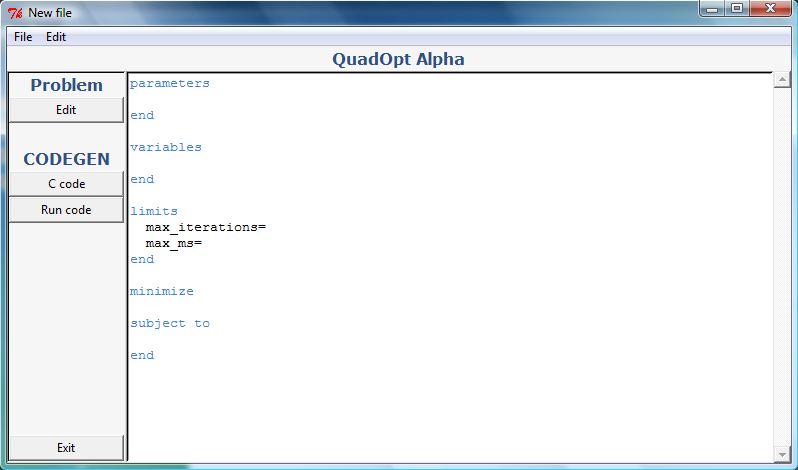
\includegraphics[scale=0.5]{bilder/gui.png}
	\end{center}
	\caption{Användargränssnittet.}
\end{figure}

